% !TEX TS-program = lualatex
%\documentclass[handout]{beamer}
\documentclass{beamer}
\input{../common/misomva}
\newcommand{\misoclasstinytitleslide}{Partially based on material by:  Ulrike von Luxburg, \\[-1em] Gary Miller, Doyle \& Schnell, Daniel Spielman}
\newcommand{\misoclassdate}{}
\usetikzlibrary{graphs}

\begin{document}
% Topic-specific title slide

\newcommand{\topictitle}{Effective Resistance Computation}

\newcommand{\topicsubtitle}{Laplacian Connection and Pseudo-Inverse}

\MakeTopicSlide

\begin{frame}
\frametitle{How to compute effective resistance?}
\pause
\rightyellbox {Kirchhoff's Law $\equiv$ flow in = flow out}
\pause
\begin{center}
% Manual layout for resistance graph (spring layout needs lualatex)
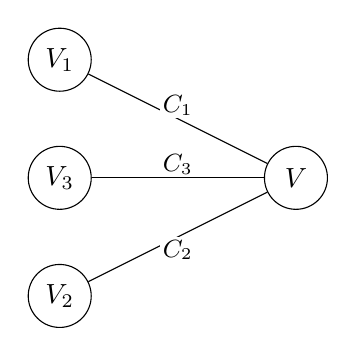
\begin{tikzpicture}[
  nd/.style={circle, draw, minimum size=8mm, inner sep=1pt},
  lbl/.style={font=\small, fill=white, inner sep=1pt, midway}]
\node[nd] (V1) at (-1.5,1.5) {$V_1$};
\node[nd] (V2) at (-1.5,-1.5) {$V_2$};
\node[nd] (V3) at (-1.5,0) {$V_3$};
\node[nd] (V) at (1.5,0) {$V$};
\draw (V1) -- node[lbl, above] {$C_1$} (V);
\draw (V2) -- node[lbl, below] {$C_2$} (V);
\draw (V3) -- node[lbl, above] {$C_3$} (V);
\end{tikzpicture}
\end{center}
\smallskip \pause
$V =  \frac{C_1}{C}V_1 +  \frac{C_2}{C}V_2 +  \frac{C_3}{C}V_3$
(convex combination)\\
\smallskip \pause
residual current = $CV - C_1V_1 - C_2V_2 - C_3V_3$ \\
 \pause Kirchhoff says: This is zero! \emphcol{There is no residual current!}
\end{frame}
%%%%%%%%%%%%%%%%%%%%%%%%%%%%%%%%%%%%%%%%%%%%%%%%%%%%%%%%%%%%%
\begin{frame}
\frametitle{Resistors: Where is the link with the Laplacian?}
\pause
\yellbox{General case of the previous!}
\pause
\smallskip
$d_i = \sum_j c_{ij} = $ sum of conductances
\pause
\[
\bL_{ij} = 
\begin{cases}
d_i & \mbox{if } i = j, \\
-c_{ij} & \mbox{if } (i,j) \in E, \\ 0 & \mbox{otherwise}. \end{cases}
\]

\pause

$\bv$ = \gcol{voltage setting} of the nodes on  graph.

\medskip \pause
$(\bL\bv)_i = $ residual current at $\bv_i$ --- as we derived
\medskip \pause \\
\textbf{Use}: setting voltages and getting the current\\
\medskip \pause
\textbf{Inverting} $\equiv$ injecting current and getting the voltages
\\ \medskip \pause
\rightyellbox{The net injected has to be zero $\equiv$ Kirchhoff's Law.}
\end{frame}
%%%%%%%%%%%%%%%%%%%%%%%%%%%%%%%%%%%%%%%%%%%%%%%%%%%%%%%%%%%%%
\begin{frame}
\frametitle{Resistors and the Laplacian: Finding $R_{\mcolA{a}\mcolC{b}}$ }

\yellbox{Let's calculate $R_{\mcolA{1}\mcolC{\nodes}}$ to get the \textbf{movie recommendation score}!} \\
\bigskip
\begin{math}
\bL \left(
\begin{array}{c}
\mcolA{0} \\
v_2 \\
\vdots \\
v_{n-1}  \\
\mcolC{1}\\
\end{array}
\right) = \left(
\begin{array}{c}
\mcolA{i} \\
0 \\
\vdots \\
0 \\
\mcolC{-i}\\
\end{array}
\right)
\end{math}

\[
i = \frac{V}{R} \qquad  V = 1 \qquad R = \frac{1}{i}
\]

Return $R_{\mcolA{1}\mcolC{\nodes}} = \dfrac{1}{i}$

\bigskip

Doyle and Snell: Random Walks and Electric Networks
{\scriptsize \url{https://math.dartmouth.edu/~doyle/docs/walks/walks.pdf}}
\end{frame}

%%%%%%%%%%%%%%%%%%%%%%%%%%%%%%%%%%%%%%%%%%%%%%%%%%%%%%%%%%%%%
\begin{frame}
\frametitle{Resistors and the Laplacian: Finding $R_{\mcolA{1}\mcolC{\nodes}}$ }

$\bL\bv = (\mcolA{i}, 0, \dots, \mcolC{-i})\transpose \equiv $ \gcol{boundary valued problem} 
\\ \bigskip \pause
For $R_{\mcolA{1}\mcolC{\nodes}}$
\\ \bigskip \pause
\qquad $V_\mcolA{1}$ and $V_\mcolC{\nodes}$ are the \gcol{boundary}
\\ \bigskip \pause
\qquad $(v_\mcolA{1}, v_2, \dots, v_\mcolC{\nodes})$ is \gcol{harmonic:}
\\ \bigskip \pause
\qquad $V_i \in$ \gcol{interior} (not boundary) 
\\ \bigskip \pause
\qquad \qquad $V_i$ is a \textbf{convex combination of its neighbors}
\end{frame}
%%%%%%%%%%%%%%%%%%%%%%%%%%%%%%%%%%%%%%%%%%%%%%%%%%%%%%%%%%%%%
\begin{frame}
\frametitle{Resistors and the Laplacian: Finding $R_{\mcolA{1}\mcolC{n}}$ }

From the properties of electric networks (cf.\@ Doyle and Snell) we inherit 
the useful properties of the Laplacians!
\\ \bigskip \pause
{\small \textbf{Example:} Semi-Supervised Learning Using Gaussian Fields and Harmonic Functions
(later in the course)}
\pause
\begin{block}{Maximum Principle}
If $\bff = \bv$ is harmonic then ${\bf\min}$ and ${\bf\max}$ are on the boundary.
\end{block}
\pause
\onslide<handout:0>{%
 \notecol{Proof: $k \in \circ \implies \exists$ neighbors $V_i, V_j$ s.t.\@ $v_i \leq v_k \leq v_j$}}
\pause
\begin{block}{Uniqueness Principle}
If $\bff$ and $\bg$ are harmonic with the same boundary then $\bff=\bg$
\end{block}
\pause
\onslide<handout:0>{%
\notecol{Proof: $\bff-\bg$ is harmonic with zero on the boundary $\implies \bff-\bg\equiv 0 \implies \bff = \bg$ (using maximum principle)}}
 \pause

\end{frame}
%%%%%%%%%%%%%%%%%%%%%%%%%%%%%%%%%%%%%%%%%%%%%%%%%%%%%%%%%%%%%
\begin{frame}
\frametitle{Resistors and the Laplacian: Finding $R_{\mcolA{1}\mcolC{\nodes}}$ }
Alternative method to calculate $R_{\mcolA{1}\mcolC{\nodes}}$: \\
\bigskip
\pause
\begin{math}
\bL\bv  = 
\left(\begin{array}{c}
\mcolA{1} \\
0 \\
\vdots \\
0 \\
\mcolC{-1}\\
\end{array}\right) \eqdef \bi_{\rm ext} \pause \quad {\rm Return} \quad R_{\mcolA{1}\mcolC{\nodes}} = v_\mcolA{1}-v_\mcolC{\nodes} \qquad
\pause \questionbox{Why?}
\end{math}
\pause \bigskip \\
\textbf{Question:} Does $\bv$ exist? \pause $\bL$ does not have an inverse :(.
\pause \\
\textbf{Not unique:} \pause $\bOne$ in the nullspace of $\bL  \pause:$  $\bL(\bv + c\bOne) = \bL\bv + c\bL\bOne = \bL\bv$  \pause
\gcol{Moore-Penrose pseudo-inverse} \pause \yellbox{solves LS} \pause \\  
\textbf{Solution:} Instead of $\bv = \bL^{-1}\bi_{\rm ext}$ we take $\bv = \bL^{+}\bi_{\rm ext}$ \\
\textbf{We get:} $R_{\mcolA{1}\mcolC{\nodes}} = v_\mcolA{1}-v_\mcolC{\nodes} = 
\bi_{\rm ext}\transpose \bv \pause =  \bi_{\rm ext} \transpose \bL^{+}  \bi_{\rm ext} $.  \pause \\
\textbf{Notice:} We can reuse $\bL^{+}$ to get resistances for any pair of nodes!
\end{frame}

%%%%%%%%%%%%%%%%%%%%%%%%%%%%%%%%%%%%%%%%%%%%%%%%%%%%%%%%%%%%%
\begin{frame}
\frametitle{What? A pseudo-inverse?}

Eigendecomposition of the Laplacian: \pause 
\[\bL = \bQ\bLambda\bQ\transpose = \pause  \sum_{i=1}^{\nodes} \lambda_i \bq_i \bq_i\transpose =  \pause  \sum_{i=2}^{\nodes} \lambda_i \bq_i \bq_i\transpose \]  
Pseudo-inverse of the Laplacian: \pause 
\[\bL^{+} = \pause  \bQ\bLambda^{+}\bQ\transpose =  \pause \sum_{i=2}^{\nodes} \frac{1}{\lambda_i} \bq_i \bq_i\transpose \]  
\gcol{Moore-Penrose pseudo-inverse}  solves a least squares problem: \pause \\  
\[\bv = \argmin_\bx \norm{\bL\bx - \bi_{\rm ext} }_2 = \pause  \bL^{+}\bi_{\rm ext}\]
\end{frame}



%%%%%%%%%%%%%%%%%%%%%%%%%%%%%%%%%%%%%%%%%%%%%%%%%%%%%%%

%%%%%%%%%%%%%%%%%%%%







\MakeLastSlide
\end{document}
